% Copyright 2019 Clara Eleonore Pavillet

% Author: Clara Eleonore Pavillet
% Description: This is an unofficial Oxford University Beamer Template I made from scratch. Feel free to use it, modify it, share it.
% Version: 1.0

\documentclass{beamer}
\usepackage{pdfpages}
% Load Packages
\usepackage[utf8]{inputenc}
\usepackage{xcolor}
\usepackage{tikz}
\usetikzlibrary{positioning,calc}
\usepackage{graphicx}
\usepackage{hyperref}
\usepackage{amsmath}
\usepackage{listings}
\usepackage{fontawesome}
\usepackage[T2A]{fontenc}
\usepackage[utf8]{inputenc}
\usepackage[russian]{babel}

% Define Commands
\newcommand*{\ClipSep}{0.06cm} %To adjust footer logo
\newcommand{\E}{\mathrm{e}\,} %\def\I{e} % used to defined e for exp(x), see later what it should be
\newcommand{\ud}{\mathrm{d}}
\lstset{numbers=left, numberstyle=\tiny, stepnumber=1,firstnumber=1,breaklines=true,
    numbersep=5pt,language=Python,
    stringstyle=\ttfamily,
    basicstyle=\footnotesize, 
    showstringspaces=false
}

\usetheme{oxonian}
\usepackage{wrapfig}
\usepackage{listings}

\title{Използване на OpenMP. Част 3.}
\subtitle{\textit{Курс „Паралелно програмиране“}}
\titlegraphic{{
\includegraphics[width=5.3cm]{iaps.png}}} 

\author{\newline \newline Стоян Мишев}

\vspace{1cm}

\date{} %\today

\begin{document}
\lstset{language=Python}
{\setbeamertemplate{footline}{} 
\frame{\titlepage}}


\section*{План}\begin{frame}{План}\tableofcontents\end{frame}

%%%%%%%%%%%%%%%%%%%%%%%%%%%%%%%%%%%%%

\section{Locks}

\begin{frame}[fragile]
  \frametitle{Locks}

  Изпълнява се нишката, която държи lock. Останалите изчакват докато се освободи. 

\begin{verbatim}
omp_init_lock()

omp_set_lock()

omp_unset_lock()

omp_destroy_lock()
\end{verbatim}
\end{frame}

\begin{frame}[plain]{Хистограма}
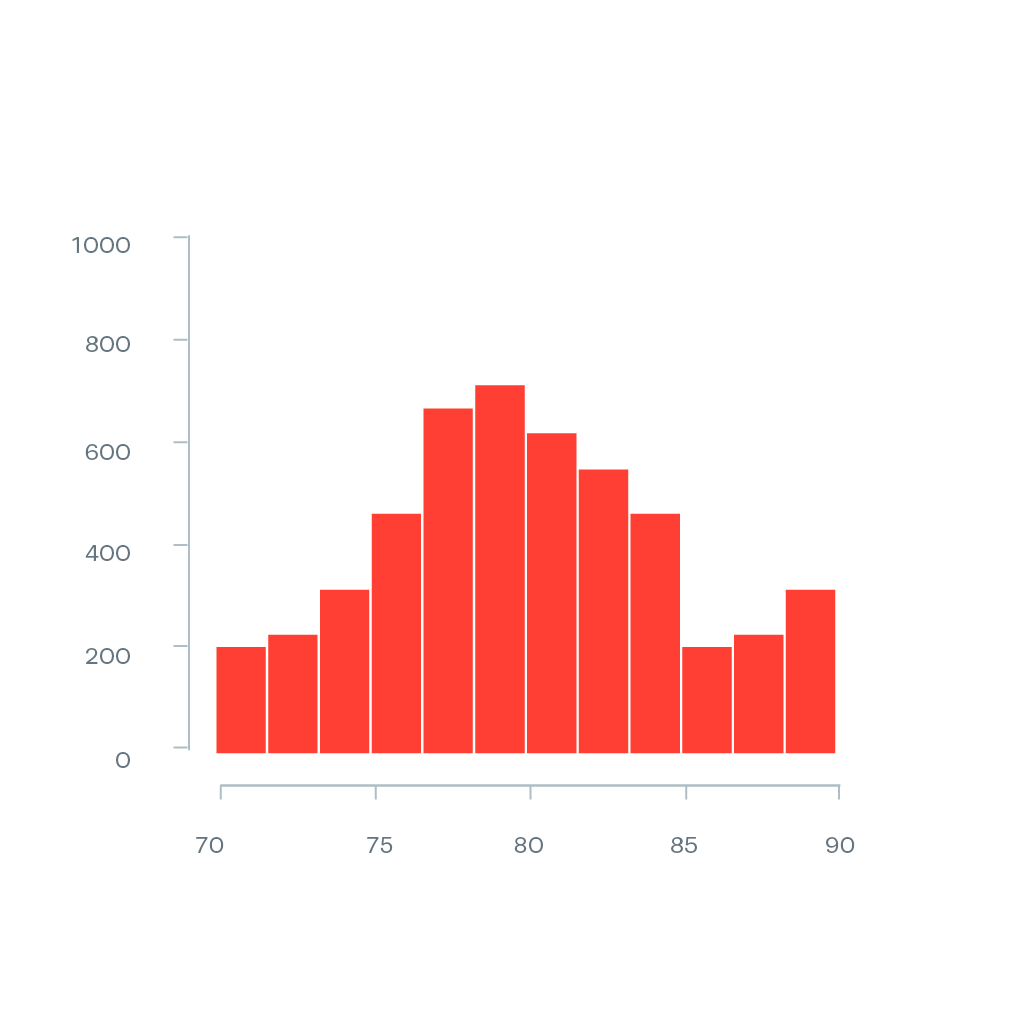
\includegraphics[width=\textwidth]{histogram}  
\end{frame}

\begin{frame}[plain]{Хистограма}
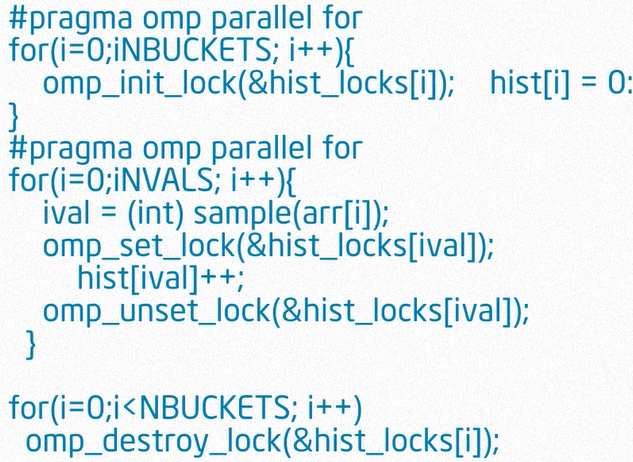
\includegraphics[width=\textwidth]{histogram_code}  
\end{frame}

\begin{frame}[fragile, plain]{Динамични директиви}
\begin{verbatim}
omp_set_num_threads()

omp_get_num_threads()

omp_get_thread_num()

omp_get_max_threads()

omp_in_parallel()

omp_set_dynamic()

omp_get_dynamic()

omp_num_procs()
\end{verbatim}  
\end{frame}

\begin{frame}
  \centering
  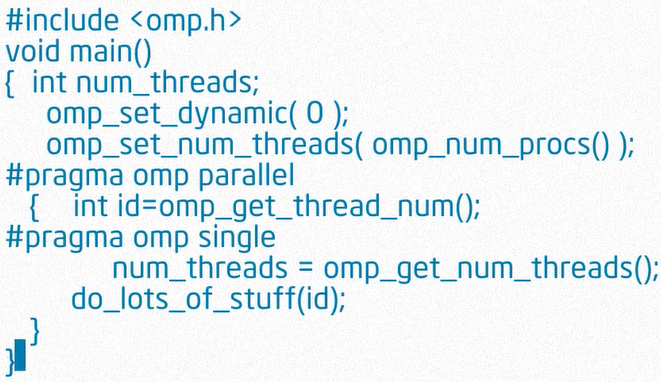
\includegraphics[height=0.7\textheight]{num-procs}
\end{frame}

\section{Shared, private, firstprivate, lastprivate}

\begin{frame}{Private}
  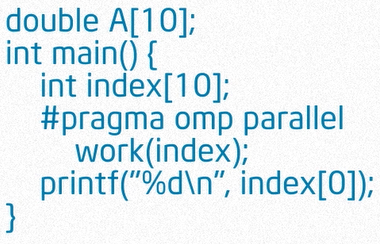
\includegraphics[height=0.3\textheight]{private}  
  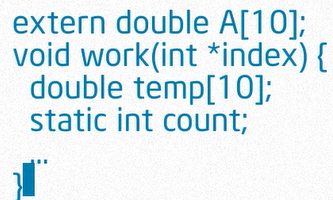
\includegraphics[height=0.3\textheight]{private2}  
  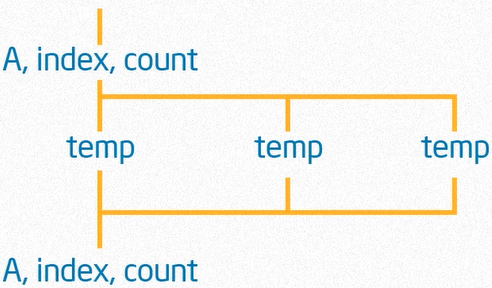
\includegraphics[height=0.17\textheight]{private3}  
\end{frame}

\begin{frame}[fragile]
\begin{verbatim}
shared

private

firstprivate

lastprivate

default(private|shared|none)
\end{verbatim}
\end{frame}


\begin{frame}{private инициализиране}
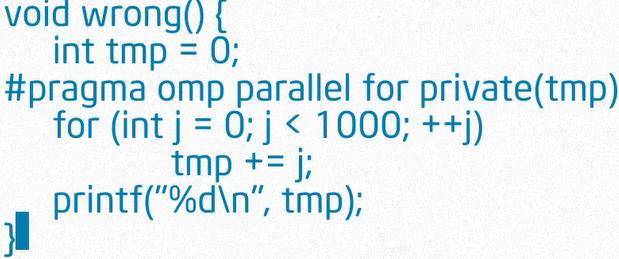
\includegraphics[width=0.6\textwidth]{private-init.png} \pause

\includegraphics[width=0.6\textwidth]{private-init2.png}
\end{frame}


\begin{frame}{private изход от паралелен блок}
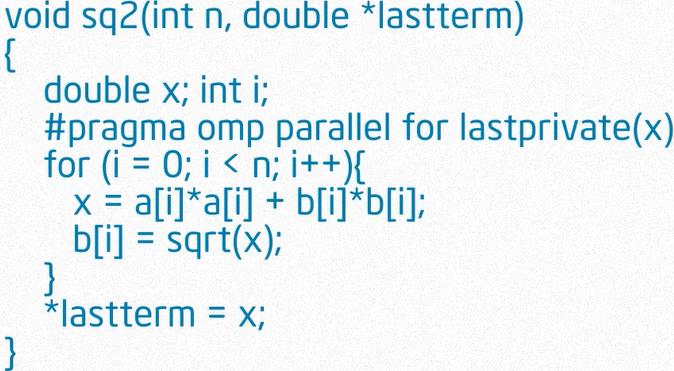
\includegraphics[width=0.6\textwidth]{private-init3.png}
\end{frame}
%\\\\\\\\\\\\\\\\\\\\\\\\\\\\\\\\\\\\\\\\\\\\\\\\\\\\\\\\\\\\\\\\\\\\\\\\\\\\\\\\\\\\\\\\\\\\\\\\\\\\\\\\\\\\\\\
\section{Примери}


\begin{frame}[plain]
  \frametitle{Площ на фрактала на Mandelbrot 1.}
  
\includegraphics[width=1.05\textwidth]{mandelbr0}
\end{frame}

\begin{frame}[plain]
  \frametitle{Площ на фрактала на Mandelbrot 2.}
  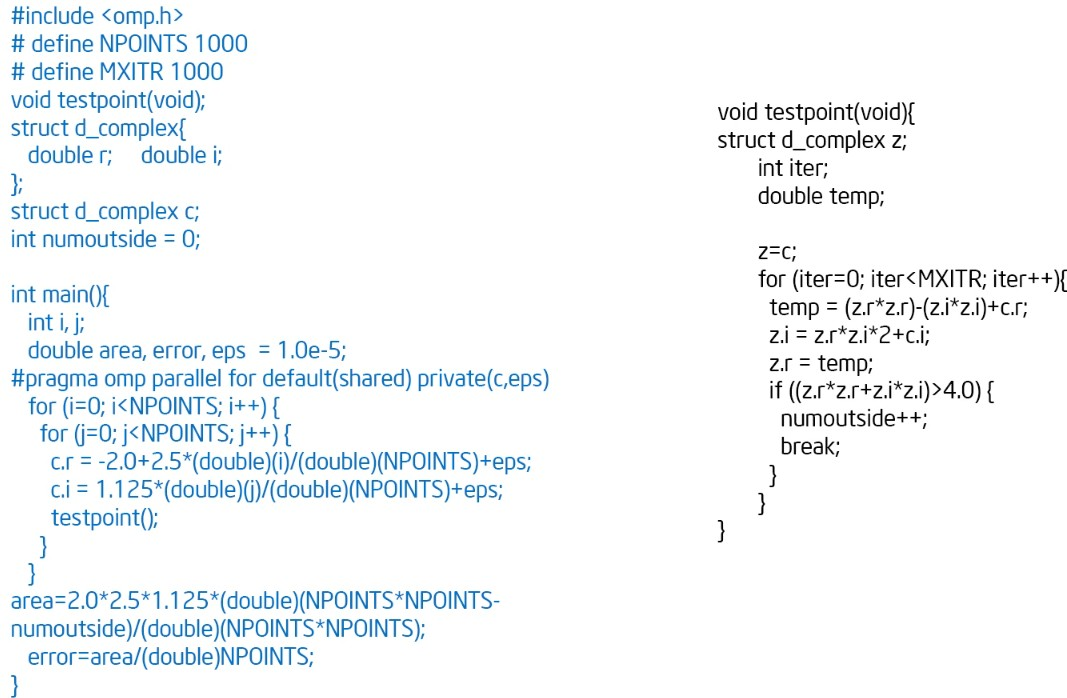
\includegraphics[width=1.07\textwidth]{mandelbr1}
\end{frame}

\begin{frame}[plain]
  \frametitle{Площ на фрактала на Mandelbrot 3.}
  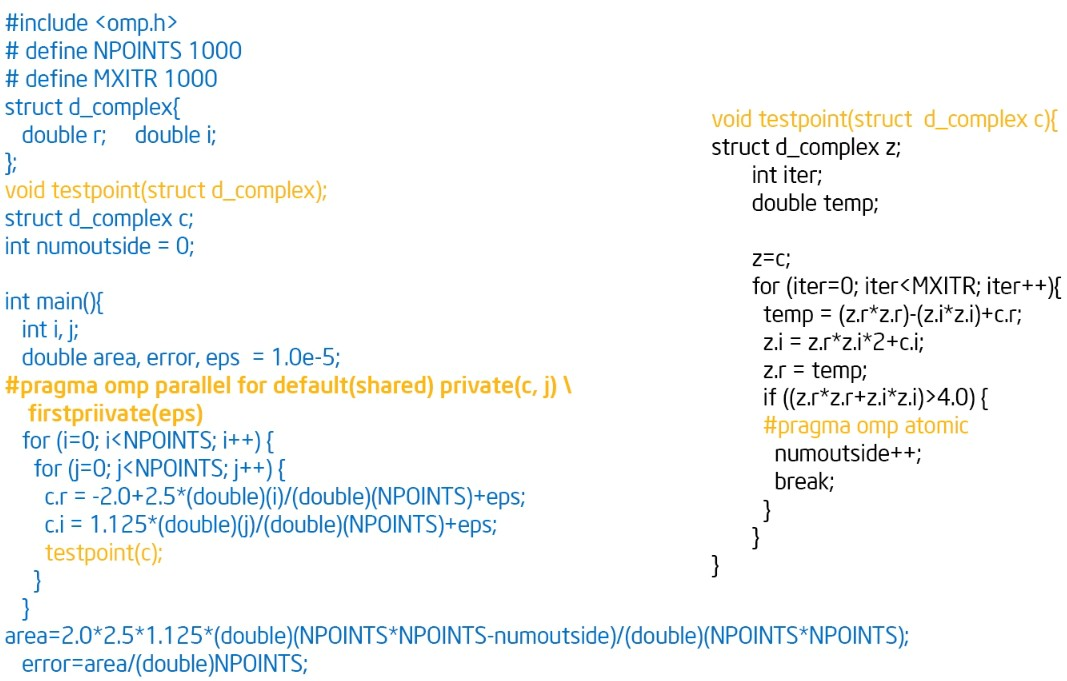
\includegraphics[width=1.07\textwidth]{mandelbr2}  
\end{frame}

%\\\\\\\\\\\\\\\\\\\\\\\\\\\\\\\\\\\\\\\\\\\\\\\\\\\\\\\\\\\\\\\\\\\\\\\\\\\\\\\\\\\\\\\\\\\\\\\\\\\\\\\\\\\\\\

\begin{frame}
  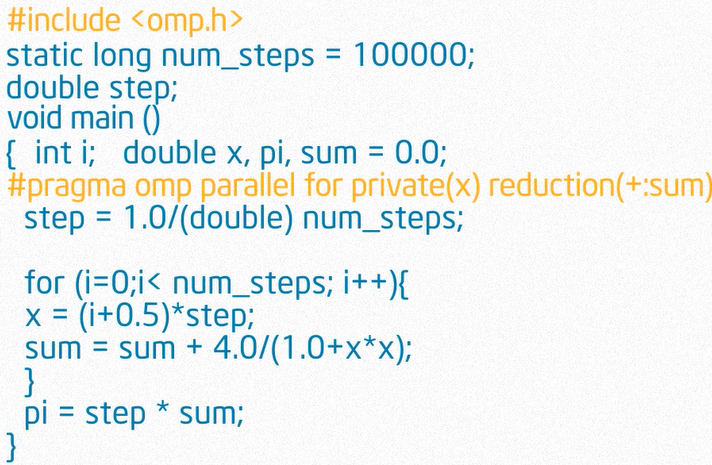
\includegraphics[width=\textwidth]{pi}
\end{frame}

\begin{frame}
  \frametitle{Домашна работа}
  от \textit{Introduction to OpenMP 11 part 2 Module 6} до \textit{Introduction to OpenMP 13 Discussion 5}

\end{frame}

\end{document}


%%% Local Variables:
%%% mode: latex
%%% TeX-master: t
%%% End:

